\documentclass[11pt]{article}
\usepackage[utf8]{inputenc}
\usepackage[spanish]{babel}
\decimalpoint
\usepackage{amsmath}
\usepackage{amsthm}
\usepackage{amssymb}
\usepackage{graphicx}
\usepackage[margin=0.8in]{geometry}
\usepackage{fancyhdr}
\usepackage[inline]{enumitem}
\usepackage{float}
\usepackage{cancel}
\usepackage{bigints}
\usepackage{listings}
\usepackage{xcolor}
\usepackage{listingsutf8}
\usepackage{algpseudocode}
\usepackage{algorithm}
\usepackage{apacite}
\usepackage{tcolorbox}
\usepackage{multicol}
\usepackage{tipa}
\usepackage{caption} 
\pagestyle{fancy}
\usepackage{hyperref}
\usepackage{mathtools}% http://ctan.org/pkg/mathtools

\hypersetup{
    colorlinks,
    citecolor=black,
    filecolor=black,
    linkcolor=black,
    urlcolor=black
}
\newcommand{\xvdash}[1]{%
	\vdash^{\mkern-10mu\scriptscriptstyle\rule[-.9ex]{0pt}{0pt}#1}%
}
\setlength{\headheight}{15pt} 
\lhead{Tarea 1. Calculo de PI}
\rhead{\thepage}
\lfoot{ESCOM-IPN}
\renewcommand{\footrulewidth}{0.5pt}
\setlength{\parskip}{0.5em}
\newcommand{\ve}[1]{\overrightarrow{#1}}
\newcommand{\abs}[1]{\left\lvert #1 \right\lvert}
\newcommand{\blank}{\text{\textcrb}}
\date{\today}
\title{Tarea 1. Calculo de PI}
\author{Sanchez Mendez Edmundo Josue}

\lstdefinestyle{customc}{
	belowcaptionskip=1\baselineskip,
	breaklines=true,
	frame=L,
	xleftmargin=\parindent,
	language=C++,
	showstringspaces=false,
	basicstyle=\ttfamily,
	keywordstyle=\bfseries\color{green!40!black},
	commentstyle=\itshape\color{purple!40!black},
	identifierstyle=\color{blue},
	numbers=left,
	stringstyle=\color{orange},
}

\lstset{escapechar=@,style=customc,tabsize=3,language=C++}

\bibliographystyle{apacite}
\begin{document}
		\begin{titlepage}
			\begin{center}
				
				% Upper part of the page. The '~' is needed because \\
				% only works if a paragraph has started.
				
				\noindent
				\begin{minipage}{0.5\textwidth}
					\begin{flushleft} \large
						
\includegraphics[width=0.5\textwidth]{resources/ipn.png}
					\end{flushleft}
				\end{minipage}%
				\begin{minipage}{0.55\textwidth}
					\begin{flushright} \large
						
\includegraphics[width=0.5\textwidth]{resources/escom.png}
					\end{flushright}
				\end{minipage}
				
				\textsc{\LARGE Instituto Politécnico Nacional}\\[0.5cm]
				
				\textsc{\Large Escuela Superior de Cómputo}\\[1cm]
				
				% Title
				
				{ \huge Tarea 1. Cálculo de PI  \\[1cm] }
				
				{ \Large Unidad de aprendizaje: Desarrollo de Sistemas Distribuidos} \\[1cm]
				
				{ \Large Grupo: 4CV11 } \\[1cm]
				
				\noindent
				\begin{minipage}{0.5\textwidth}
					\begin{flushleft} \large
						\emph{Alumno:} \\
						Sanchez Mendez Edmundo Josue
					\end{flushleft}
				\end{minipage}%
				\begin{minipage}{0.5\textwidth}
					\begin{flushright} \large
						\emph{Profesor:} \\
						Pineda Guerrero Carlos 
					\end{flushright}
				\end{minipage}
				
				\vfill
				% Bottom of the page
				{\large {\today}}
			\end{center}
		\end{titlepage}
	
	\titlepage
	\tableofcontents
	\newpage
	
	\section{Introducción}
		Mediante el desarrollo de un sistema distribuido la cual tendrá una topología lógica de estrella, se hará un cálculo aproximado del número PI haciendo uso de la serie de Gregory-Leibniz, la cual esta definida de la siguiente manera.
		 \[ \pi
  = 4(1 -
  \dfrac{1}{3} + 
  \dfrac{1}{5} - 
  \dfrac{1}{7} + ...) = 4 \sum_{n=0}^{\infty}\dfrac{(-1)^{n}}{2n+1} 
\]
	En donde los denominadores son los números impares y el signo negativo se va alternando entre cada miembro de la suma. El sistema distribuidos contara con 5 nodos que se ejecutaran en una misma computadora, en donde uno de los 5 nodos sera el servidor y el encargado de mostrar el valor aproximado calculado por el sistema, mientras que los 4 nodos restantes actuaran como los clientes serán los encargados de hacer los cálculos correspondientes.
	\section{Desarrollo}
Una vez programado el sistema distribuido con base en los algoritmos establecidos en la tarea se procedió a realizar la compilación de un archivo con nombre PI.java el cual se encuentra en el archivo comprimido que se entrego en la plataforma.
		\subsection{Compilación del código}
		En la figura 1 podemos ver como la compilación de nuestro programa PI.java se hace de manera exitosa y sin ningún error alguno, esto desde el Símbolo del sistema (CMD) de Windows 10.
		\begin{figure}[H]
			\centering
			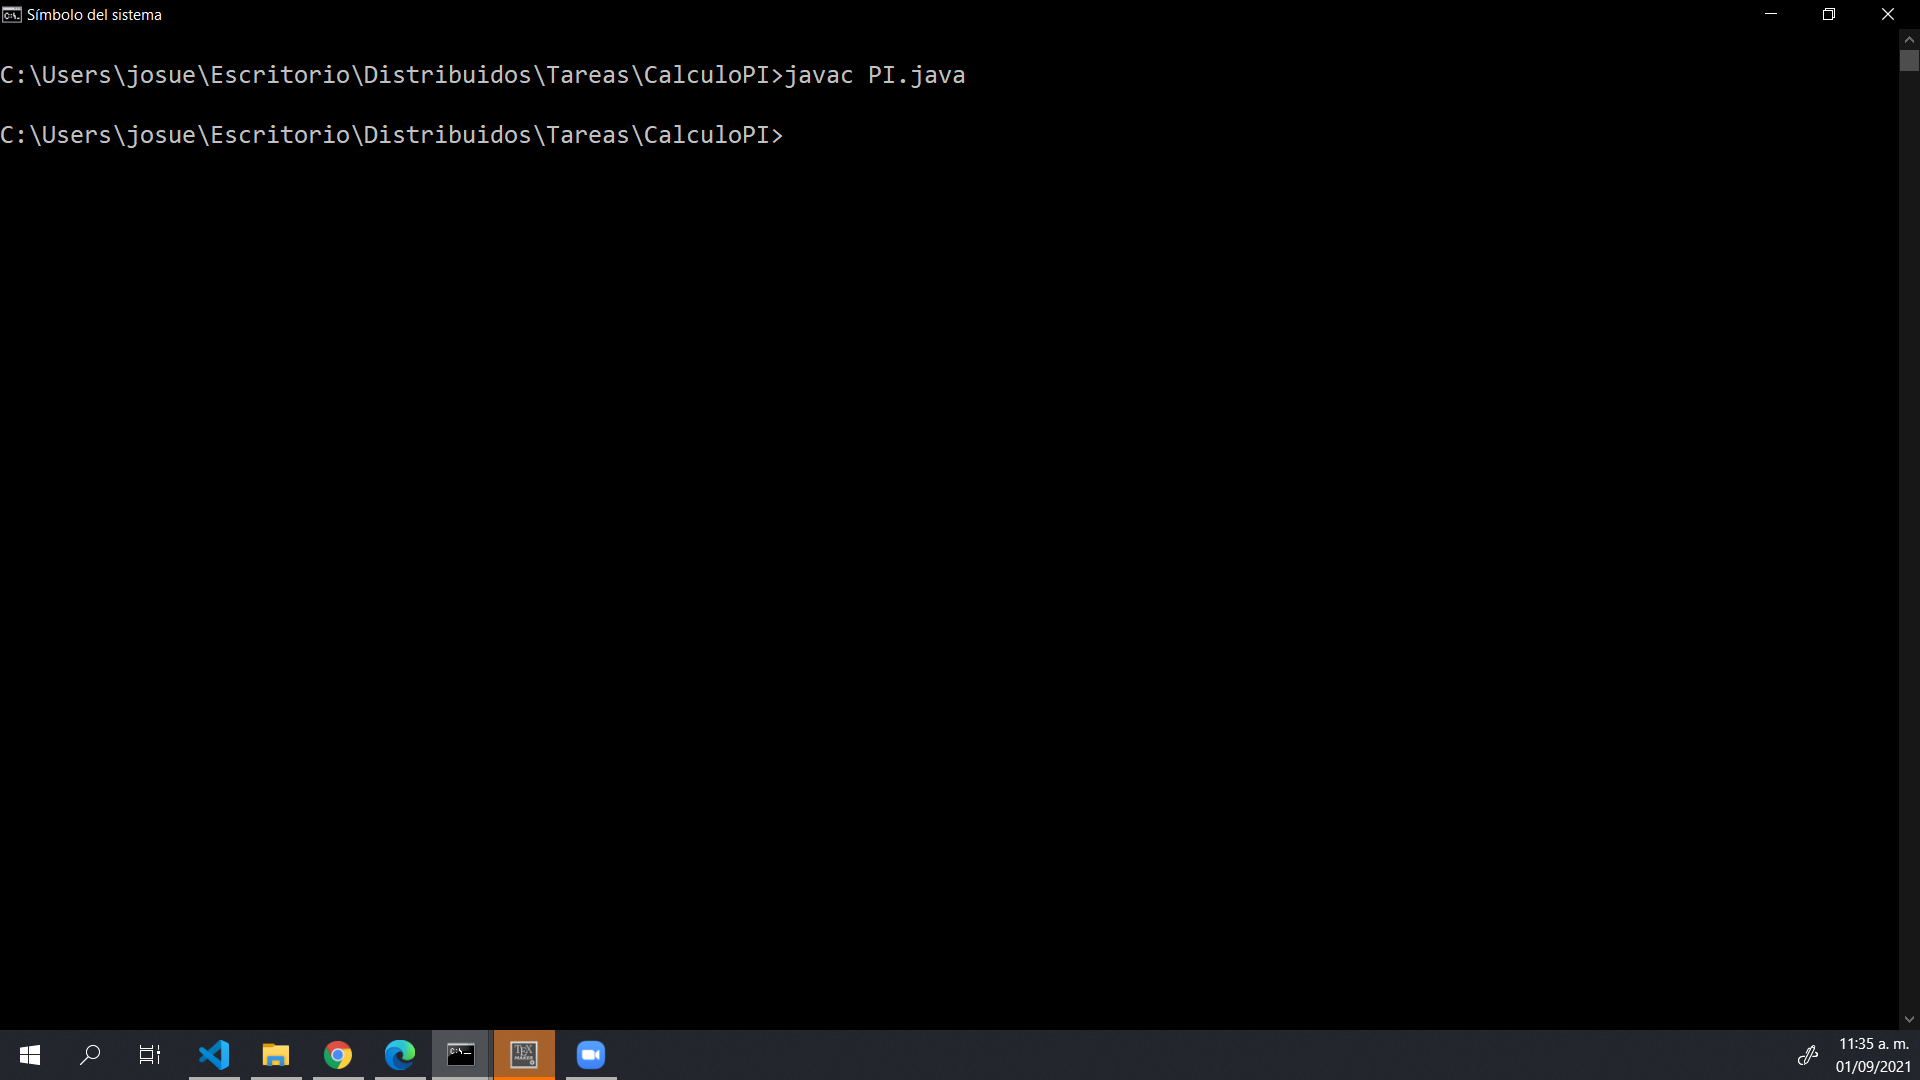
\includegraphics[scale=0.34]{resources/compilacionpi.png}
			\caption{Compilación del código por medio de CMD. }\label{fig:picture}
		\end{figure}
		\subsection{Ejecución del programa}
		Primero ejecutamos el nodo del servidor, para ello se le pasa al programa el valor 0, desde
la consola:
		\begin{figure}[H]
			\centering
			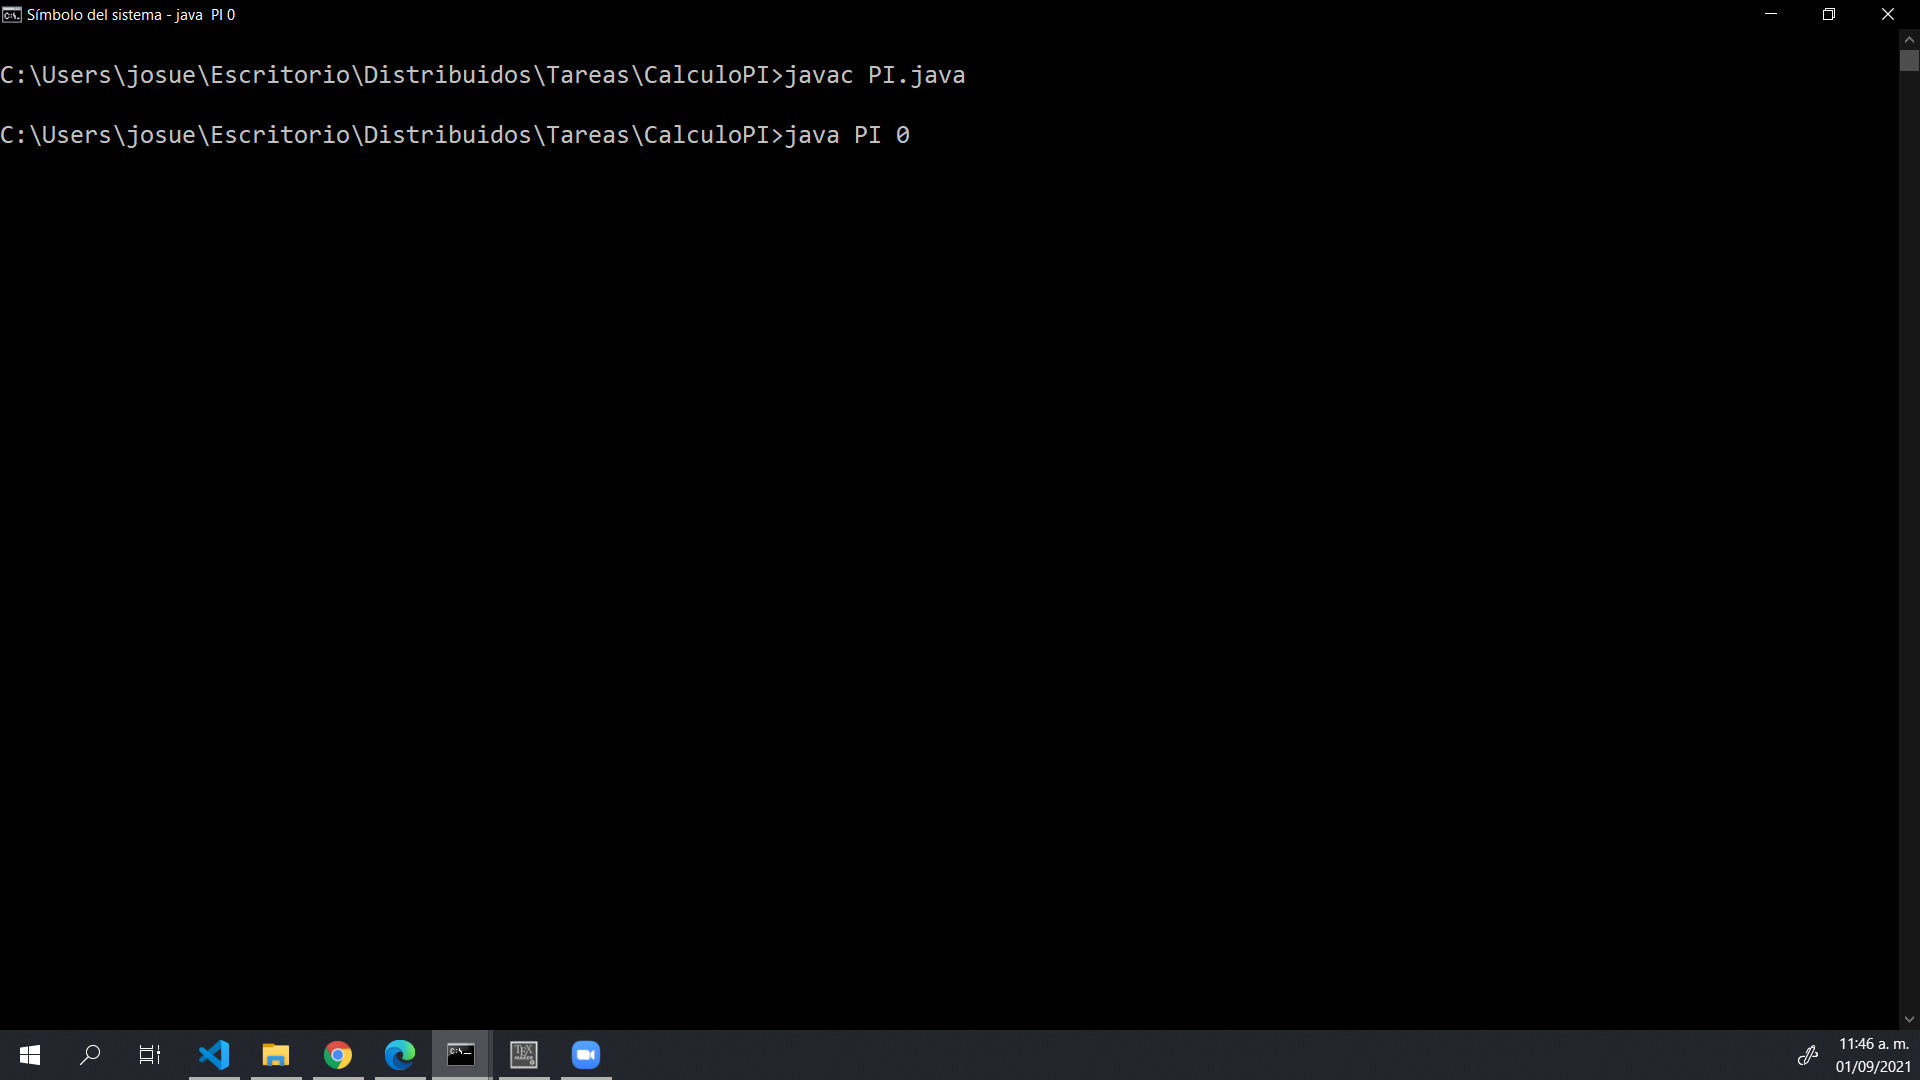
\includegraphics[scale=0.34]{resources/nodo0.png}
			\caption{Ejecución del Nodo 0 de nuestro sistema distribuido. }\label{fig:picture}
		\end{figure}
		Después abrimos 4 nuevas terminales y ejecutamos a los 4 clientes, pasando el valor de 1, 2, 3, 4 a cada terminal para poder completar el numero total de nodos requeridos en nuestro sistema distribuido:
		\begin{figure}[H]
			\centering
			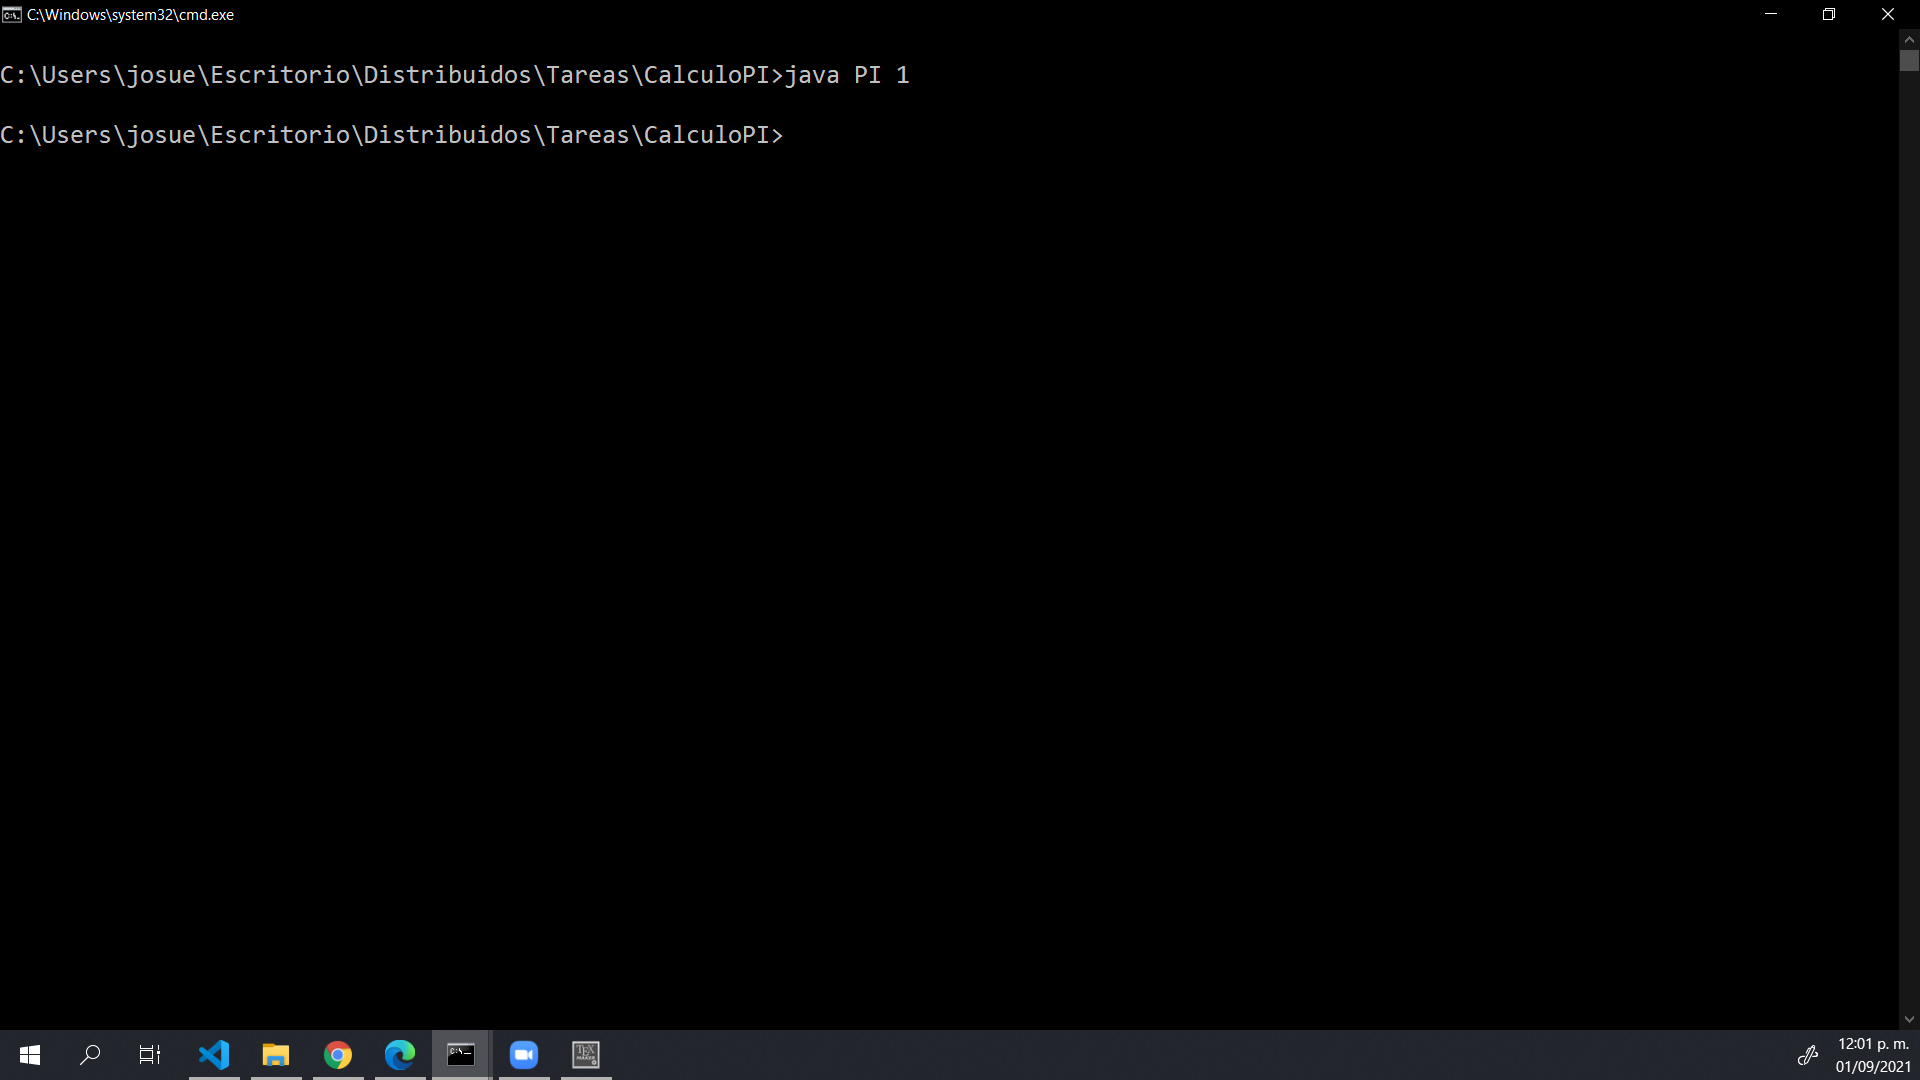
\includegraphics[scale=0.34]{resources/nodo1.png}
			\caption{Ejecución del nodo 1 de nuestro sistema distribuido. }\label{fig:picture}
		\end{figure}
		\begin{figure}[H]
			\centering
			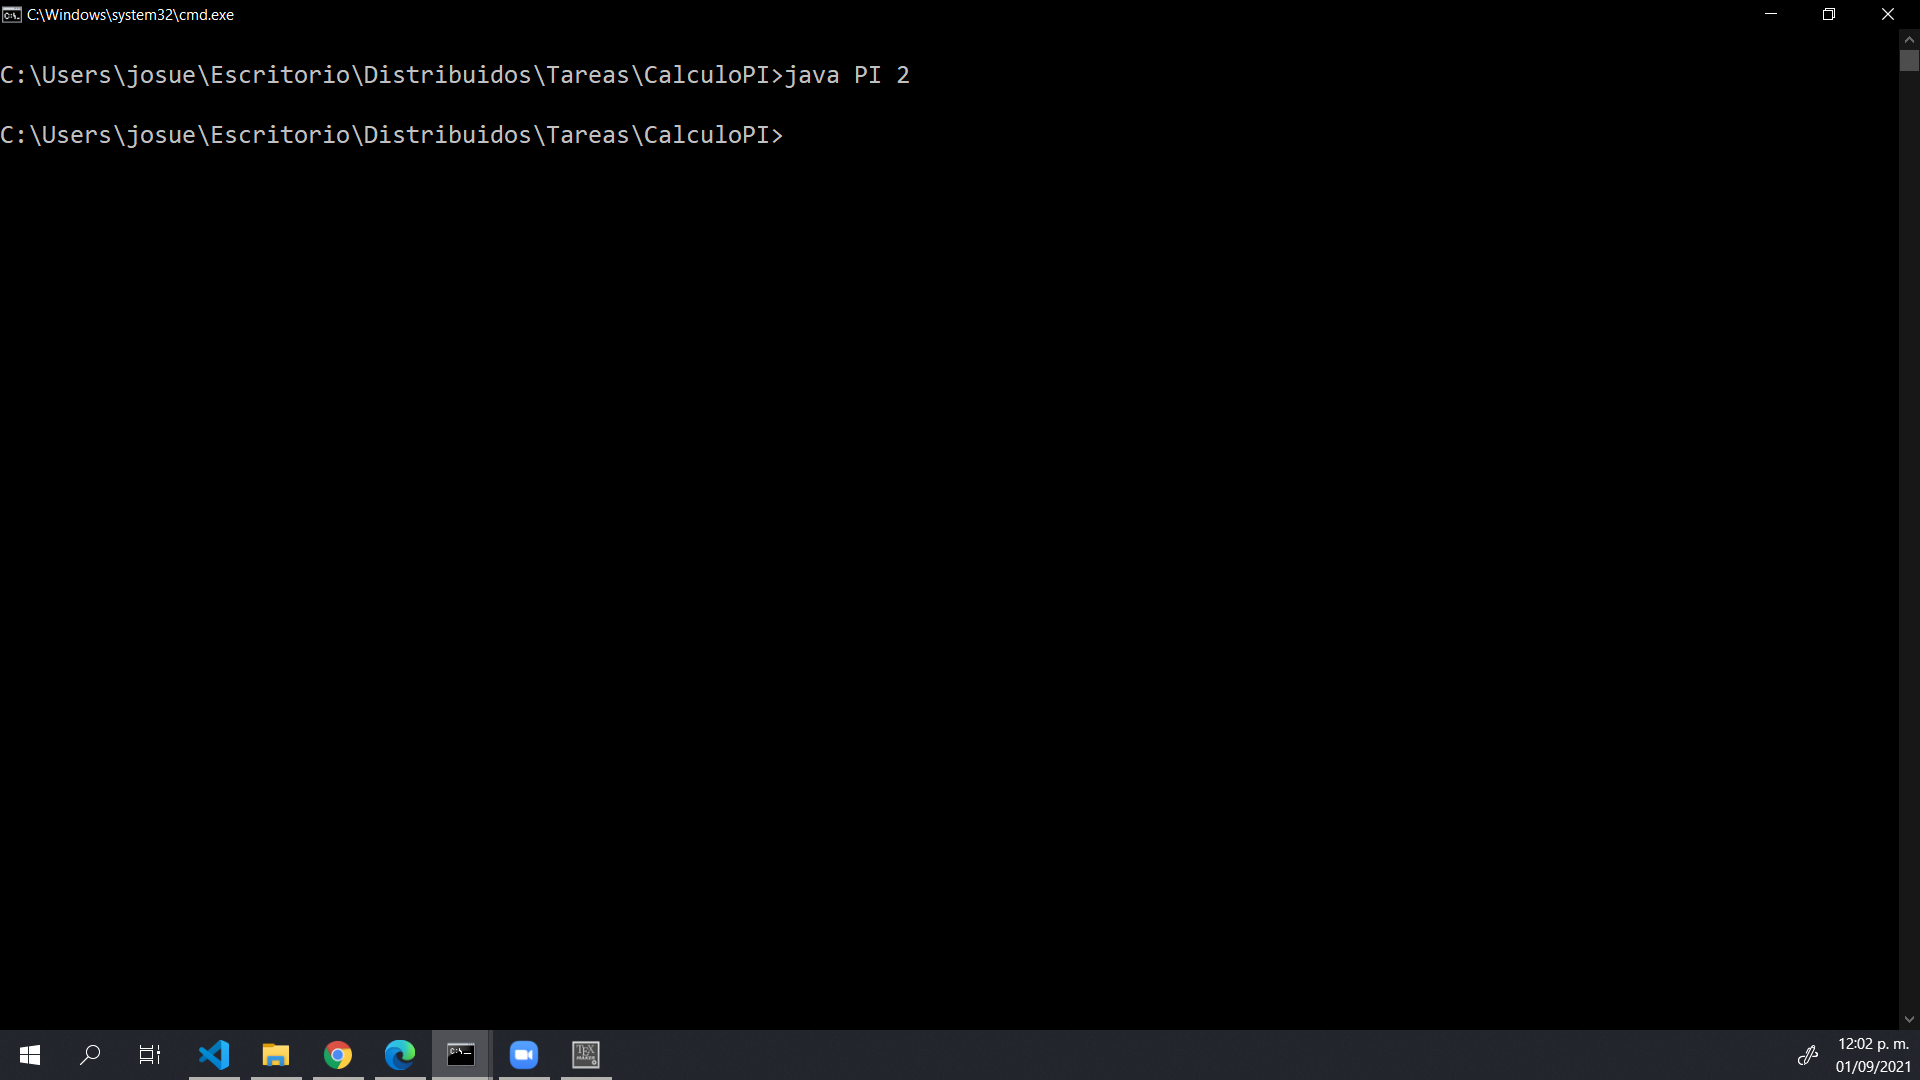
\includegraphics[scale=0.34]{resources/nodo2.png}
			\caption{Ejecución del nodo 2 de nuestro sistema distribuido. }\label{fig:picture}
		\end{figure}
		\begin{figure}[H]
			\centering
			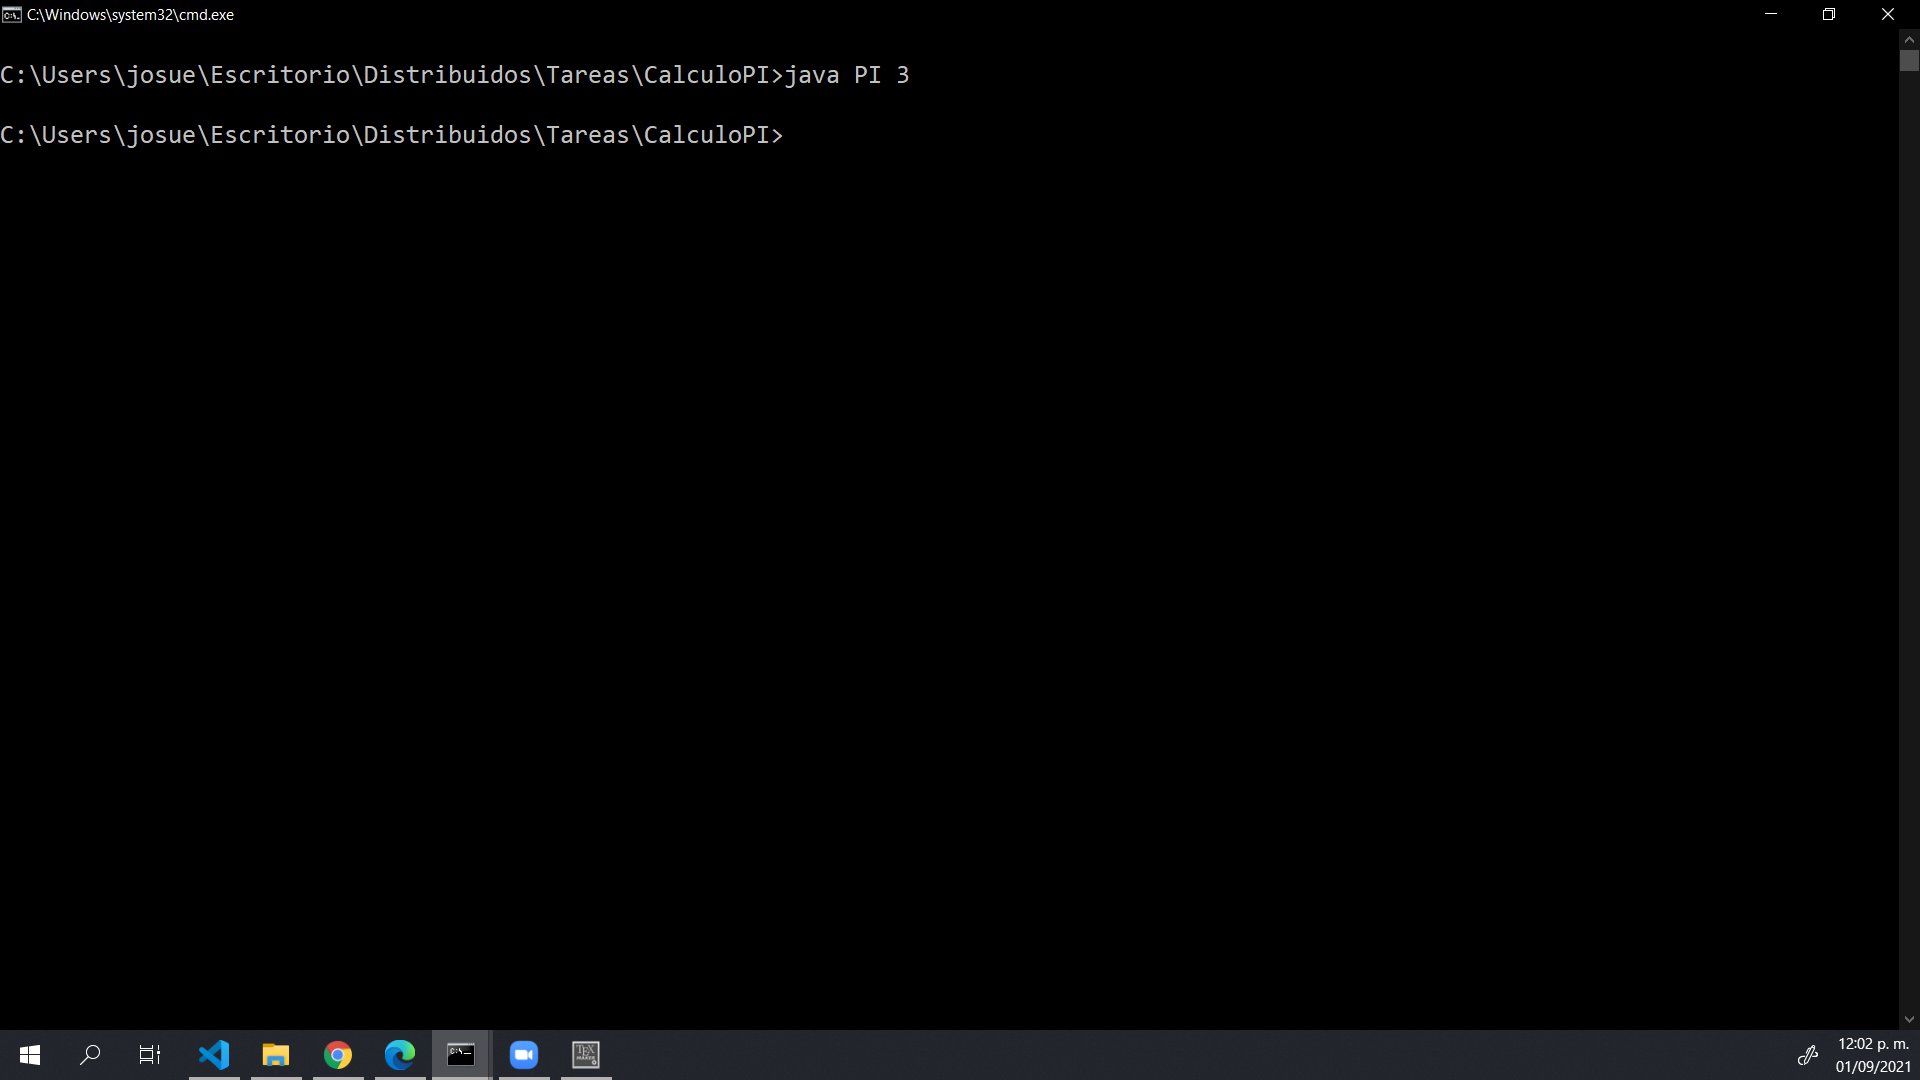
\includegraphics[scale=0.34]{resources/nodo3.png}
			\caption{Ejecución del nodo 3 de nuestro sistema distribuido. }\label{fig:picture}
		\end{figure}
		\begin{figure}[H]
			\centering
			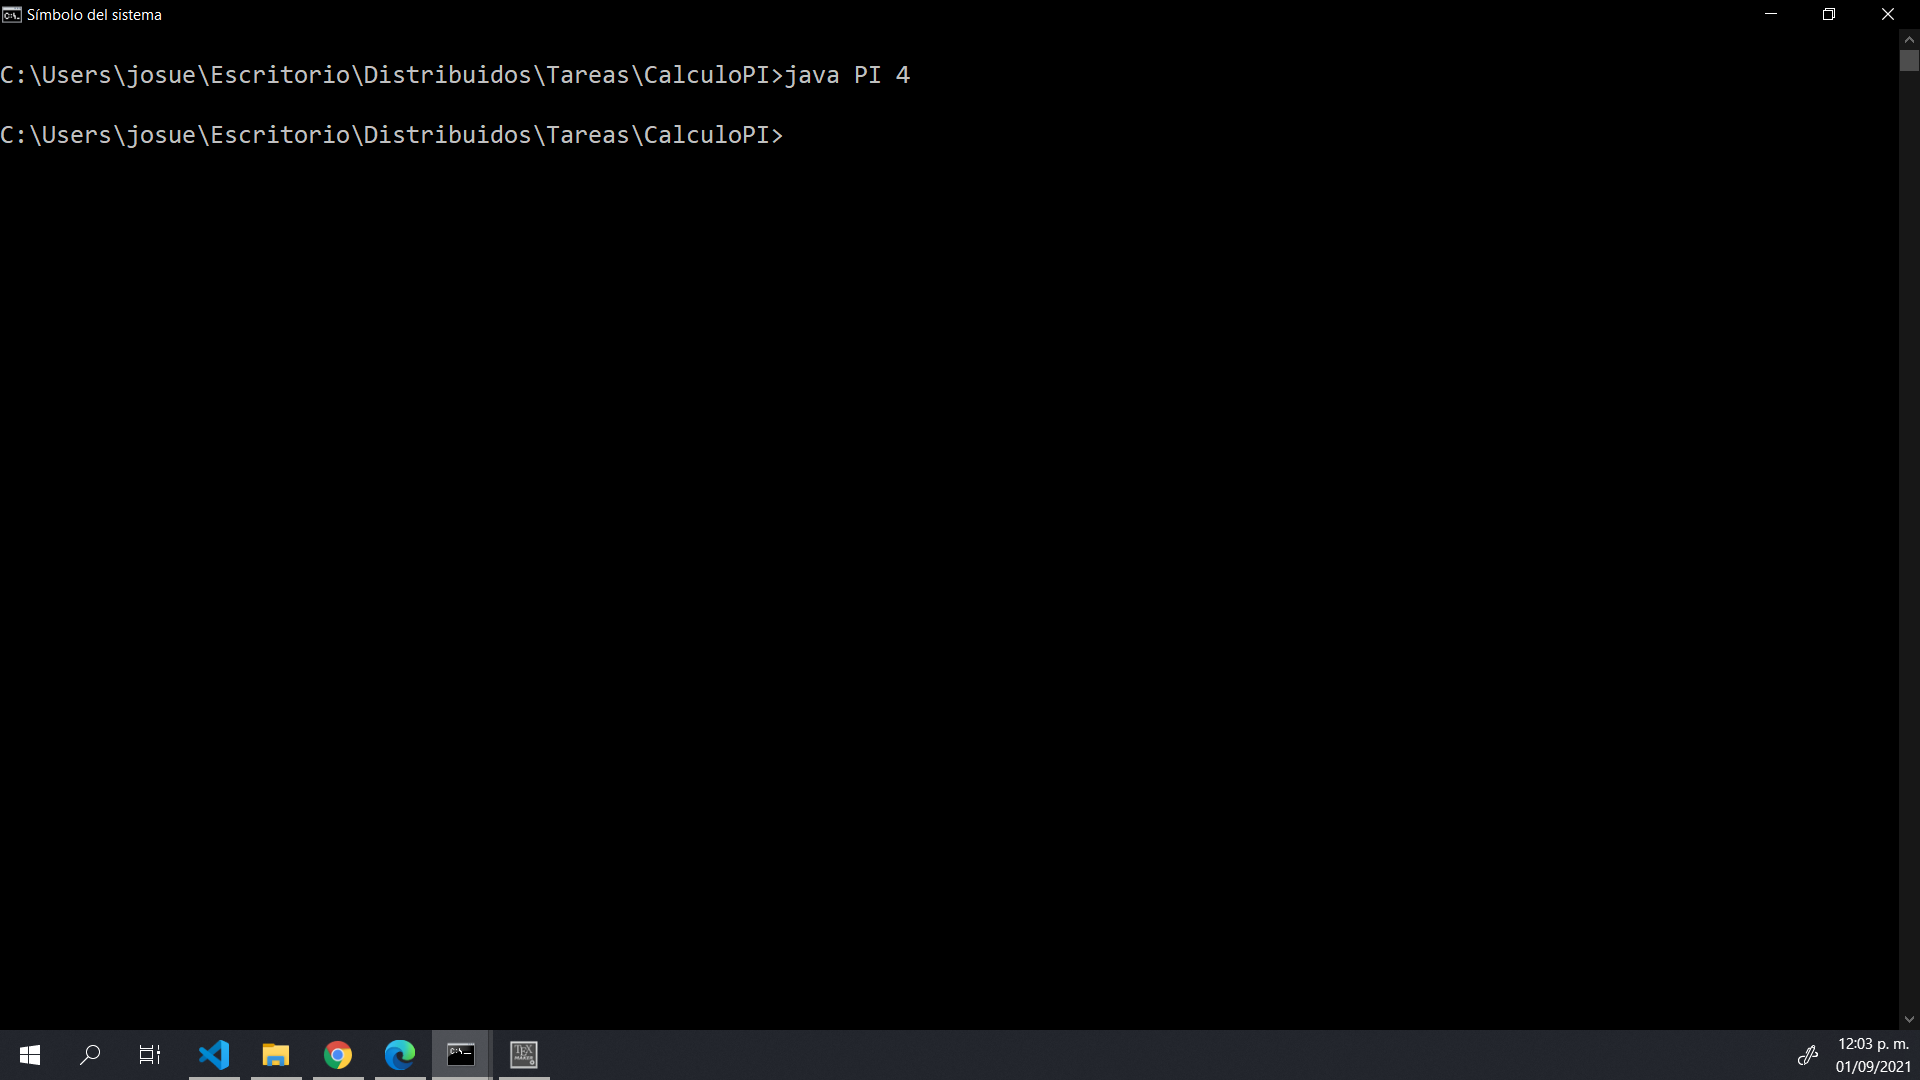
\includegraphics[scale=0.34]{resources/nodo4.png}
			\caption{Ejecución del nodo 4 de nuestro sistema distribuido. }\label{fig:picture}
		\end{figure}
		Cuando se ejecute al último cliente, la consola en donde esta el servidor mostrará el resultado obtenido de PI, el cual es el mostrado en la figura 7:
		\begin{figure}[H]
			\centering
			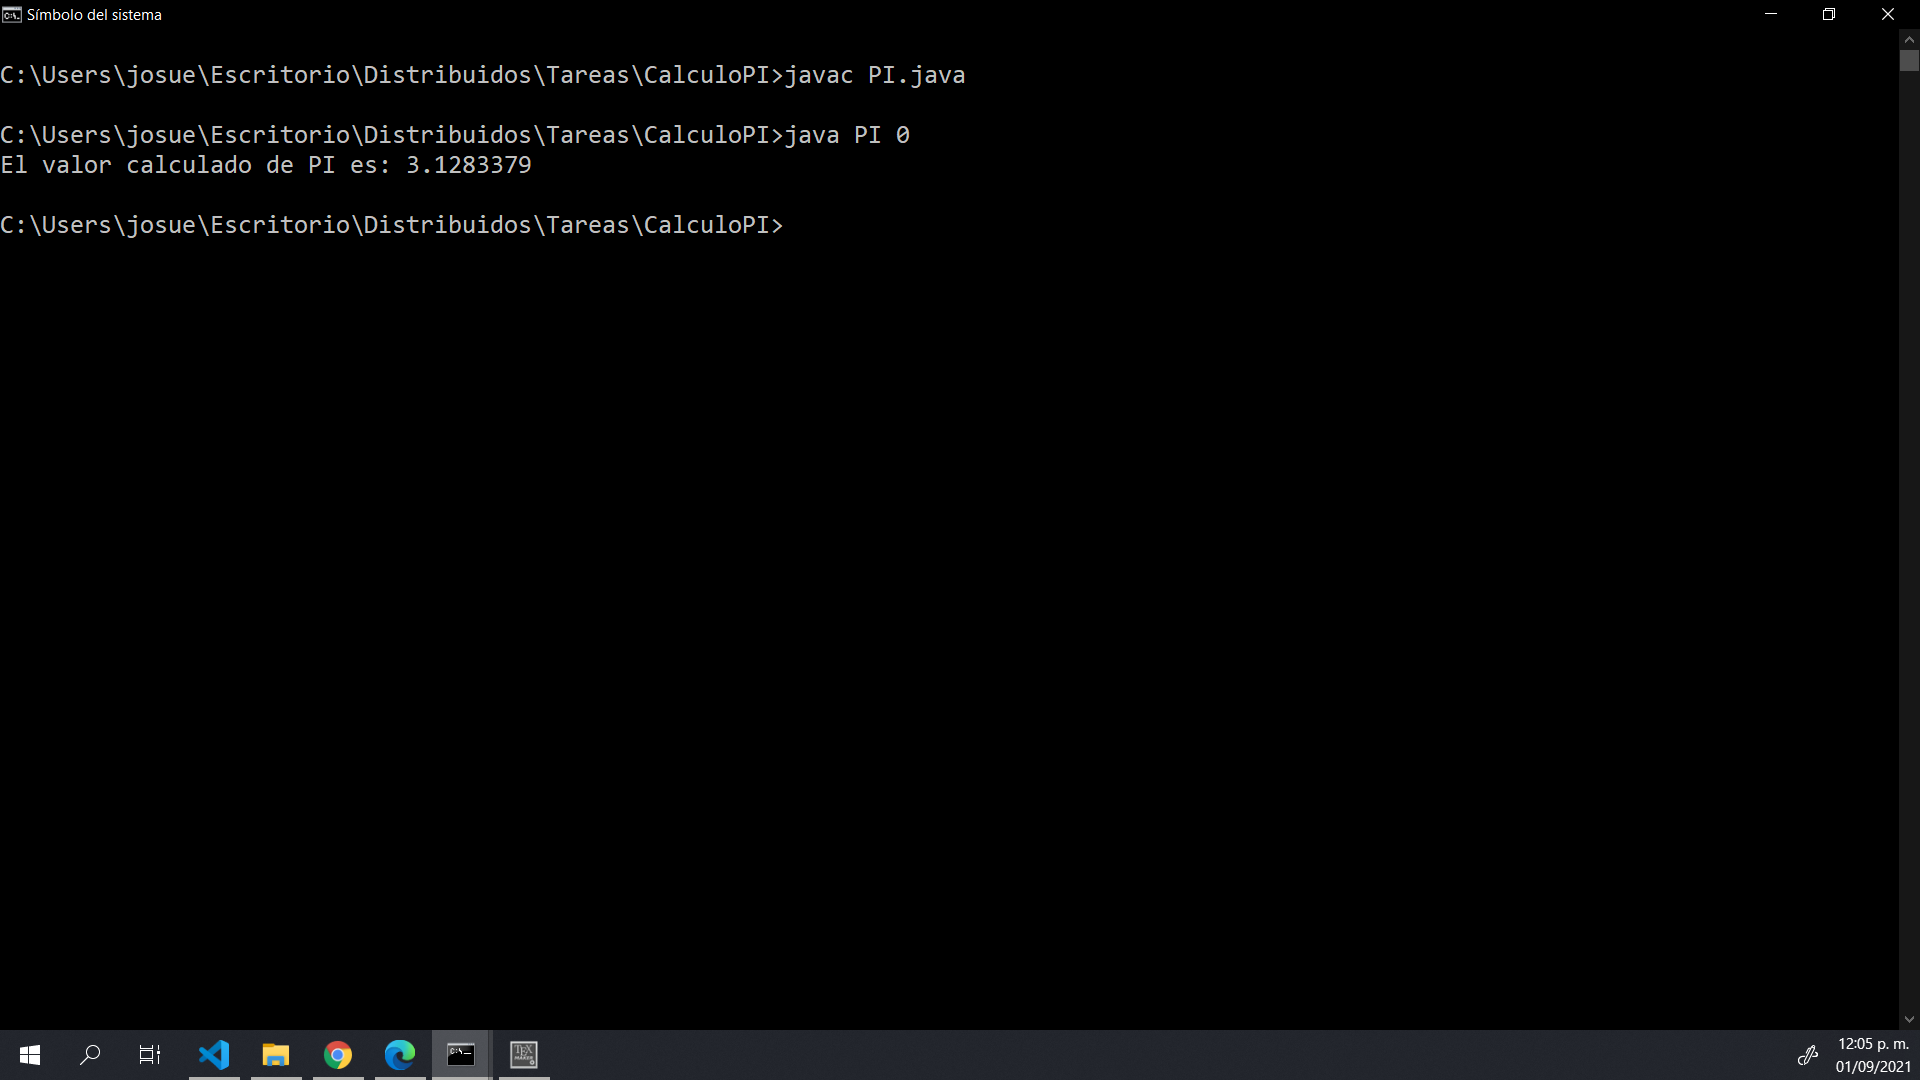
\includegraphics[scale=0.34]{resources/resultado.png}
			\caption{Valor arrojado por nuestro sistema distribuido. }\label{fig:picture}
		\end{figure}
	\section{Conclusiones}
	Esta tarea me ayudo a recordar los conocimientos de la materia de materias anteriores como redes 2 en el uso de java para aplicaciones de comunicaciones en red y conocimientos de redes 1 haciendo uso de una topología de tipo estrella, también un recordatorio en el uso de hilos y de herramientas para sincronizar los mismos, además de darme una pequeña introducción a los sistemas distribuidos, viendo cómo podemos dividir el trabajo haciendo uso distintos procesos o hilos para poder reducir el tiempo de ejecución. Finalmente comentar que el valor calculado de PI seria mas próximo al valor establecido de PI si usáramos el tipo de dato double en lugar de usar float esto debido a que double nos proporciona de 15 a 16 décimas en comparación con el tipo de dato float que nos proporciona de 6 a 7 décimas, es decir, double nos proporciona mayor cantidad de información la cual en este caso es útil para tener una mayor aproximación al valor de PI.
	\begin{thebibliography}{1}
 \bibitem[label1]{cite_key1} WLynn, B. (s. f.). Pi - The Gregory-Leibniz Series. Applied Cryptography Group | Stanford University. https://crypto.stanford.edu/pbc/notes/pi/glseries.html [Accessed 01 September 2021].
\end{thebibliography}

\end{document}
